
\documentclass[11pt,a4paper]{article}
\usepackage[T1]{fontenc}
\usepackage{lmodern}
\usepackage[margin=21mm]{geometry}
\usepackage{graphicx,booktabs,tabularx,float,caption,xcolor,fancyhdr}
\usepackage[colorlinks=true,urlcolor=blue,pdfusetitle]{hyperref}
\definecolor{navy}{HTML}{17365A}
\setlength{\parindent}{0pt}
\setlength{\parskip}{7pt}
\setlength{\headheight}{15pt}
\renewcommand{\arraystretch}{1.25}
\captionsetup{font=small,labelfont=bf,hypcap=false}
\pagestyle{fancy}
\fancyhf{}
\fancyfoot[L]{\small ResilientBite \enspace $\cdot$ \enspace Project report}
\fancyfoot[R]{\small Page \thepage}
\renewcommand{\headrulewidth}{0pt}
\newcommand{\phase}[1]{\section*{\textcolor{navy}{#1}}}
\newcommand{\topic}[1]{\subsection*{\textcolor{navy}{#1}}}
\title{ResilientBite}
\author{Karthik Kavuri, Akula Sai Teja, and Muvvala Harsha Vardhan}
\date{}
\begin{document}
\begin{center}
\vspace*{27mm}
{\Large\bfseries IIITDM KANCHEEPURAM\par}
\vspace{3mm}
{\large IDSE Project\par}
\vspace{15mm}
{\Huge\bfseries ResilientBite\par}
\vspace{6mm}
{\Large Campus Food Demand Forecasting\par}
\vspace{11mm}
{\large Analysis and Application Report\par}
\vspace{12mm}
{\large\bfseries Team Members\par}
\vspace{3mm}
\begin{tabular}{@{}l@{\qquad}l@{}}
Karthik Kavuri & CS24I1025 \\
Akula Sai Teja & CS24I1054 \\
Muvvala Harsha Vardhan & EC24B1019
\end{tabular}\par
\vspace{22mm}
Prepared from the supplied ResilientBite master dataset
\end{center}
\clearpage
\phase{Contents and scope}
ResilientBite forecasts daily demand for each dish, meal and dining hall. We evaluated whether the forecast could improve on using demand from the same day last week. We then simulated two ways a kitchen could use the forecast to decide how many portions to prepare.

\begin{tabularx}{\linewidth}{@{}cXr@{}}
\toprule
\textbf{Section} & \textbf{Topic} & \textbf{Page} \\
\midrule
1 & Dataset and demand & 2 \\
2 & Data quality and cleaning & 2 \\
3 & Exploratory data analysis & 3 \\
4 & Forecast inputs and date splits & 4 \\
5 & Model training and test results & 4 to 5 \\
6 & Food preparation simulation & 6 \\
7 & Application & 7 \\
8 & Conclusions & 8 \\
\bottomrule
\end{tabularx}
\phase{1. Dataset and demand}
The supplied CSV describes a campus dining scenario in Chennai. Each row represents a dish at one meal and dining hall on one date. Demand is measured as served portions plus unmet portions. Preparation records let us compare predicted demand with the quantities already prepared.

\begin{tabularx}{\linewidth}{@{}p{.31\linewidth}X@{}}
\toprule
\textbf{Property} & \textbf{Observed value} \\
\midrule
Records and columns & 32,850 records and 30 columns \\
Dates & 1 January to 30 December 2024 across 365 dates \\
Coverage & 3 dining halls, 3 meal types and 30 dishes \\
\bottomrule
\end{tabularx}
\phase{2. Data quality and cleaning}
We parsed dates, converted portion counts and calendar flags to numbers, and trimmed spaces from hall and meal labels. The checks looked for duplicate rows, missing values, invalid counts and inconsistent totals. Demand had to equal portions served plus unmet demand. Preparation had to equal portions served plus leftovers. All 32,850 original rows passed. We verified the cleaning function on a separate practice file, where it removed five of 11 rows containing intentional errors.


\clearpage
\phase{3. Exploratory data analysis}
We explored the earliest 60\% of dates before comparing the models. The charts show demand per dish, how daily totals changed, which meals usually required more portions, and the difference between vacation and other days.

\begin{figure}[H]
\centering
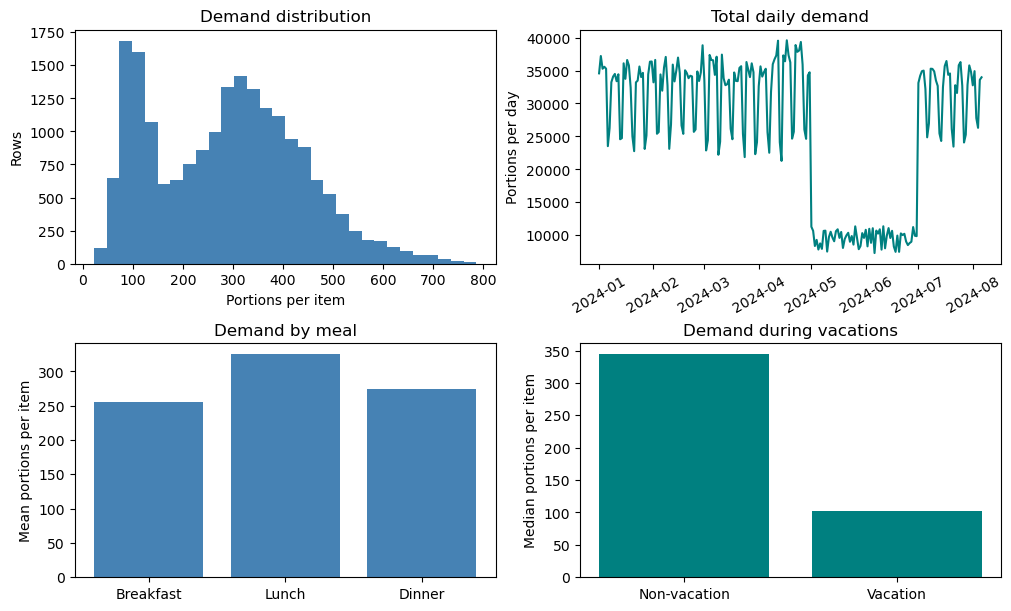
\includegraphics[width=\linewidth]{images/demand.png}
\caption{Demand patterns on the exploratory dates.}
\end{figure}
\topic{Patterns in the data}
Lunch had the highest mean demand at about 325 portions per item. Median demand was 103 portions during vacations and 344 on other days. Daily totals also fell in May and June, when the dataset flags vacation dates. These patterns supported using a vacation flag as a forecast input.

We flagged unusually high demand using the upper quartile plus 1.5 times the spread between the upper and lower quartiles. Eleven records exceeded the resulting threshold of about 763 portions. Their portion totals were consistent, so we kept them to represent busy meals that the kitchen needs to plan for.


\clearpage
\phase{4. Forecast inputs and date splits}
The forecast uses demand from yesterday and from seven days earlier for the same dish, meal and hall. The other three inputs indicate weekends, vacations and exams. Actual attendance and preparation may only be known later, so the model uses information available before service.

We split the dates chronologically, with roughly 60\% for training, 20\% for validation and 20\% for testing. The first week supplied historical values and was left out of model fitting. During testing, each day used only earlier demand, as it would when forecasting after the previous day's totals were recorded.

\begin{tabularx}{\linewidth}{@{}lXr@{}}
\toprule
\textbf{Period} & \textbf{Dates in 2024} & \textbf{Rows} \\
\midrule
Training & 8 January to 6 August & 19,080 \\
Validation & 7 August to 18 October & 6,570 \\
Test & 19 October to 30 December & 6,570 \\
\bottomrule
\end{tabularx}
\phase{5. Model training and test results}
The baseline repeats demand from seven days earlier. Linear Regression combines the five inputs in an equation. Random Forest averages 60 decision trees and can capture patterns such as changes in how useful recent demand is during vacations. Depths of 4, 8 and 12 gave validation errors of 58.97, 55.99 and 56.86 portions. We selected depth 8 before evaluating the test dates.

\begin{tabularx}{\linewidth}{@{}Xrrrr@{}}
\toprule
\textbf{Model} & \textbf{Validation MAE} & \textbf{Test MAE} & \textbf{Test RMSE} & \textbf{Test R\textsuperscript{2}} \\
\midrule
Last week & 65.41 & 81.63 & 113.19 & 0.34 \\
Linear regression & 59.18 & 60.58 & 76.16 & 0.70 \\
Random Forest & 55.99 & 51.91 & 66.72 & 0.77 \\
\bottomrule
\end{tabularx}
MAE averages absolute misses. RMSE gives larger misses more weight. Both use portions. R\textsuperscript{2} compares performance with predicting the same constant for every row.

Random Forest had the lowest error on validation and test. Its test MAE of 51.91 portions was 36.4\% lower than the weekly baseline across 73 test dates.


\clearpage
\phase{5. Model training and test results continued}
\topic{Where the forecast missed}
\begin{figure}[H]
\centering
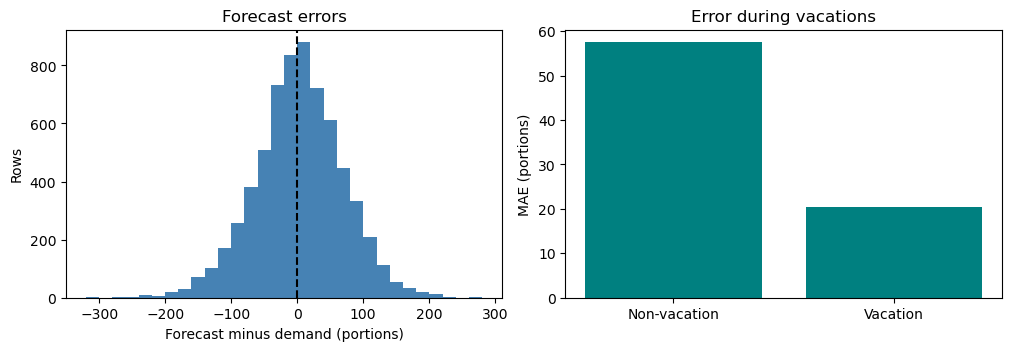
\includegraphics[width=\linewidth]{images/errors.png}
\caption{Forecast errors overall and by vacation status.}
\end{figure}
\begin{tabularx}{\linewidth}{@{}Xrrr@{}}
\toprule
\textbf{Test period} & \textbf{Rows} & \textbf{MAE} & \textbf{Mean signed error} \\
\midrule
Outside vacation & 5,580 & 57.48 & +3.85 \\
Vacation & 990 & 20.50 & 2.66 below zero \\
\bottomrule
\end{tabularx}
Signed error is forecast minus demand. Positive values indicate an overestimate.

On days outside vacation, the forecast missed by 57.48 portions on average and tended to overestimate. During vacation, it missed by 20.50 portions and tended to underestimate. Vacation accounted for 990 of 6,570 test rows. The overall average signed error was an overestimate of 2.87 portions, which can hide differences between the two groups.

The largest miss was Chicken Biryani at lunch in Dining Hall B on 25 November. Demand was 728 portions and the forecast was about 408. That miss matters for kitchen planning because a low average error can still include substantial shortages on individual dishes.


\clearpage
\phase{6. Food preparation simulation}
We compared recorded preparation with the forecast rounded up and with the forecast increased by 10\% before rounding. For every test row, we calculated excess when preparation exceeded demand and unmet portions when demand exceeded preparation. The simulation used the same observed demand under all three rules.

\begin{tabularx}{\linewidth}{@{}Xrr@{}}
\toprule
\textbf{Preparation rule} & \textbf{Mean excess} & \textbf{Mean unmet} \\
\midrule
Recorded preparation & 6.61 & 6.25 \\
Forecast only & 27.64 & 24.29 \\
Forecast + 10\% & 47.48 & 12.20 \\
\bottomrule
\end{tabularx}
Average portions per dish, meal and hall on the test dates.

\begin{figure}[H]
\centering
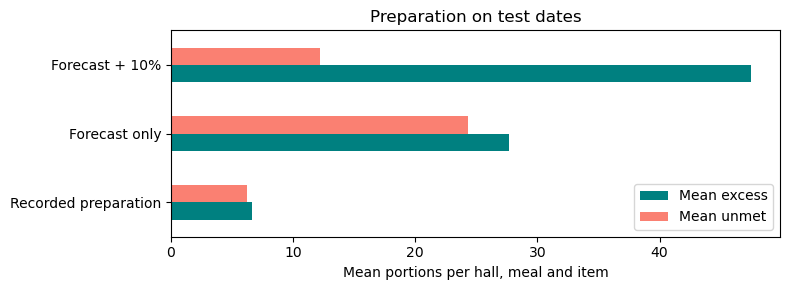
\includegraphics[width=\linewidth]{images/preparation.png}
\caption{Excess and unmet portions by preparation rule.}
\end{figure}
The buffer lowered unmet demand from 24.29 to 12.20 portions compared with the unbuffered forecast. Excess rose from 27.64 to 47.48. Recorded preparation had the lowest average excess and unmet demand of the three rules tested.

This simulation measures portions above or below demand. A kitchen trial would need to weigh food waste separately and assess whether shortages affect what diners request.


\clearpage
\phase{7. Application}
The web and Android apps accept CSV and Excel files. For today's forecast, include the scheduled dishes and their actual demand from yesterday and seven days ago. The app displays predicted portions by dish, meal and hall, and lets users filter or download the results. Historical demo mode uses the 2024 dataset.

The Android APK connects over HTTPS to the Python app hosted on Render. The app uses the same training period, Random Forest settings and five inputs as the notebook. Forecasts require internet access in the Android app.

\topic{Android app demonstration}
The demo CSV contains 288 rows. It provides demand history from 8 to 14 November 2026 and a menu of 36 rows for 15 November across three halls. The demonstration uses dates shifted from the original dataset. The submission ZIP contains both CSVs.

The app predicted 9,646 portions across all 36 menu rows. The results screenshot shows the table filtered to Dining Hall A. The total above the table still covers all three halls.


\noindent
\begin{minipage}[t]{0.48\linewidth}
\centering
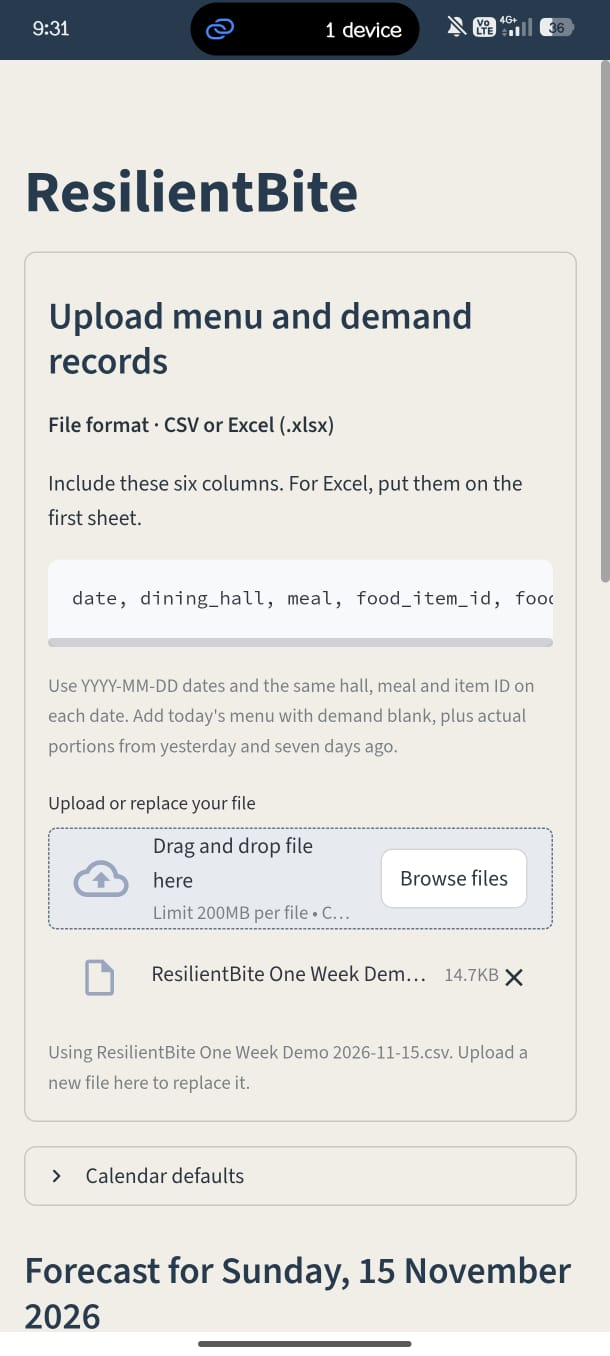
\includegraphics[width=54mm]{images/android-upload.jpg}
\captionof{figure}{The demo CSV loaded in the Android app.}
\end{minipage}\hfill
\begin{minipage}[t]{0.48\linewidth}
\centering
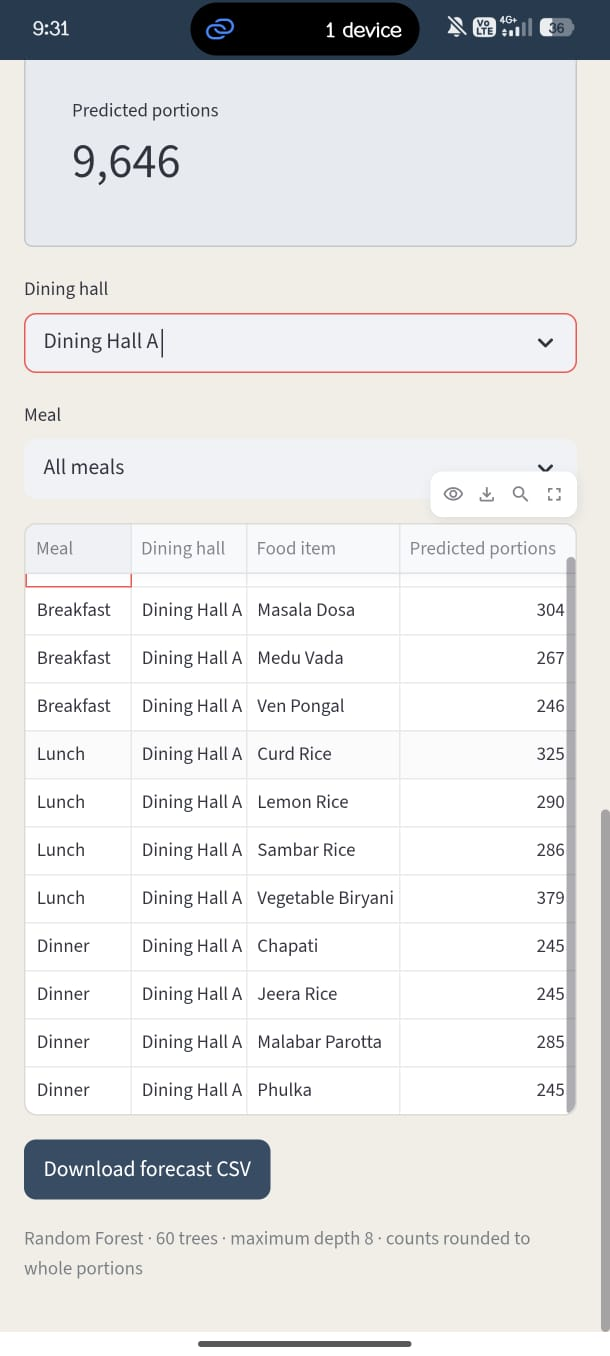
\includegraphics[width=54mm]{images/android-results.jpg}
\captionof{figure}{Predicted portions filtered to Dining Hall A.}
\end{minipage}

\clearpage
\phase{8. Conclusions}
Random Forest improved on the weekly forecasting baseline. The preparation simulation showed that better demand estimates alone did not improve both kitchen outcomes. The recorded preparation quantities provide a reference for evaluating future preparation rules.

\topic{Limitations and next steps}
The supplied CSV covers one year, three halls and a fixed menu. The collection method is undocumented. The model also relies on recent demand being recorded on time. Testing on a later term and measuring shortages and waste separately in a kitchen trial would help establish whether the approach transfers to daily use.

\topic{Reproducing the results}
The project folder contains the original dataset, the analysis notebook, a README and a list of package versions. The Random Forest uses a fixed seed of 42. Two independent notebook runs generated identical results tables.


\topic{Project links}
\href{https://res-b7z8.onrender.com}{Hosted forecasting app}\par
\href{https://github.com/Hackerliongloi/ResilientBite/releases/tag/v1.6}{Android release}\par
\href{https://github.com/Hackerliongloi/ResilientBite}{Source repository}\par

\end{document}
